% ieeeaccess.cls reuses \year as a metadata setter. Preserve the TeX primitive
% so PGF/TikZ can initialize its deterministic machinery while loading.
\let\PSevenTeXYear\year
\documentclass{ieeeaccess}

% Shared packages and notation. Do not change IEEE Access class formatting here.
\usepackage{cite}
\usepackage{amsmath,amssymb,amsfonts}
\usepackage{graphicx}
\usepackage{textcomp}
\usepackage{bm}
\usepackage{booktabs}
\usepackage{array}
\usepackage{tabularx}
\usepackage{xcolor}
% The legacy IEEE Access class encodes its blue as a Pantone spot color that
% some current PDF renderers drop. Preserve the journal hue in device RGB so
% titles, section heads, and captions remain visible in archival renderers.
\definecolor{accessblue}{RGB}{0,114,178}
\let\PSevenIEEEAccessYear\year
\let\year\PSevenTeXYear
\usepackage{tikz}
\let\year\PSevenIEEEAccessYear
\usetikzlibrary{arrows.meta,positioning,fit,calc,shapes.geometric,backgrounds}
\usepackage[hidelinks]{hyperref}
\usepackage{etoolbox}

% ieeeaccess.cls adds an unnumbered REFERENCES entry to the PDF outline after
% creating the heading. Supply its hyperlink destination without altering the
% official class or its visual bibliography formatting.
\makeatletter
\patchcmd{\thebibliography}{\section*{\refname}}{\section*{\refname}\phantomsection}{}{}
\makeatother

% Replace the class template's published-volume placeholder with an honest
% circulation marker. The official class file itself remains unmodified.
\newcommand{\PSevenDraftFooter}{PREPRINT}
\makeatletter
\patchcmd{\ps@titlepage}{\footervolfont VOLUME\ \thevol, \theyear}{\footervolfont\PSevenDraftFooter}{}{}
\patchcmd{\ps@titlepage}{\footervolfont VOLUME\ \thevol, \theyear}{\footervolfont\PSevenDraftFooter}{}{}
\patchcmd{\ps@headings}{\footervolfont VOLUME\ \thevol, \theyear}{\footervolfont\PSevenDraftFooter}{}{}
\patchcmd{\ps@headings}{\footervolfont VOLUME\ \thevol, \theyear}{\footervolfont\PSevenDraftFooter}{}{}
\AtBeginDocument{\ps@headings}
\makeatother

\newtheorem{proposition}{Proposition}
\newtheorem{definition}{Definition}
\newtheorem{corollary}{Corollary}

\DeclareMathOperator*{\argmax}{arg\,max}
\DeclareMathOperator*{\argmin}{arg\,min}
\newcommand{\R}{\mathbb{R}}
\newcommand{\Pset}{\mathcal{P}}
\newcommand{\Hset}{\mathcal{H}}
\newcommand{\given}{\,|\,}

% Writing-assistance attribution, separate from scientific-source citations.
\newcommand{\AIDraftingCredit}{\footnote{Drafting/revision assistance:
OpenAI Codex~\cite{openaiCodex2026}.}}

\usepackage{pdfpages}
\usepackage{placeins}
\newcommand{\ObservedPMUCount}{8}
\newcommand{\HiddenBusCount}{31}
\newcommand{\NominalTestCount}{100}
\newcommand{\BZeroTVE}{0.3402\%}
\newcommand{\BOneTVE}{0.009904\%}
\newcommand{\BTwoTVE}{0.009634\%}
\newcommand{\BTwoRelativeImprovement}{2.7\%}
\newcommand{\BTwoMinusBOnePP}{-0.000270}
\newcommand{\BTwoMinusBOneCILowPP}{-0.000359}
\newcommand{\BTwoMinusBOneCIHighPP}{-0.000179}
\newcommand{\BTwoWinRate}{69.0\%}
\newcommand{\FunctionalSpearman}{0.5625}
\newcommand{\FunctionalSpearmanCILow}{0.271}
\newcommand{\FunctionalSpearmanCIHigh}{0.751}
\newcommand{\FunctionalPermutationP}{0.0012}
\newcommand{\FunctionalKendall}{0.376}
\newcommand{\MismatchMainCount}{980}
\newcommand{\MismatchRefinementCount}{175}
\newcommand{\NetworkMismatchRatio}{16.99}
\newcommand{\OperatingMismatchRatio}{8.32}
\newcommand{\OnlineClosurePercent}{0.4\%}
\newcommand{\UtwoNLL}{-16.184}
\newcommand{\UtwoCoverageRe}{93.9\%}
\newcommand{\UtwoCoverageIm}{94.2\%}
\newcommand{\OriginalInnovationACF}{0.602}
\newcommand{\MeasurementGMInnovationACF}{0.540}
\newcommand{\MismatchUzeroCoverage}{92.9\%}
\newcommand{\MismatchUtwoCoverage}{47.5\%}
\newcommand{\AdequacyHalfAUROC}{0.901}
\newcommand{\AdequacyHalfAUPRC}{0.779}
\newcommand{\AdequacyMaxAUROC}{0.928}
\newcommand{\AdequacyMaxAUPRC}{0.787}
\newcommand{\NetworkFrozenTVE}{0.250430\%}
\newcommand{\NetworkOracleTVE}{0.002547\%}
\newcommand{\NetworkOnlineTVE}{0.251132\%}
\newcommand{\OperatingFrozenTVE}{0.122641\%}
\newcommand{\OperatingOracleTVE}{0.001006\%}
\newcommand{\OperatingOnlineTVE}{0.122381\%}
\newcommand{\CoupledFrozenTVE}{0.023615\%}
\newcommand{\CoupledOracleTVE}{0.000396\%}
\newcommand{\CoupledOnlineTVE}{0.023615\%}
\newcommand{\EZeroHDevCount}{30}
\newcommand{\EZeroHTestCount}{60}
\newcommand{\EZeroHValidRate}{100.0\%}
\newcommand{\EZeroHClosureOverall}{98.1\%}
\newcommand{\EZeroHRuntimeMedian}{61.7}
\newcommand{\EZeroHRuntimePNinetyFive}{76.0}
\newcommand{\EZeroHRank}{25}
\newcommand{\EZeroHDimension}{43}
\newcommand{\EZeroHNullity}{18}
\newcommand{\EZeroHFunctionalResidual}{0.0419}
\newcommand{\EZeroHFrozenHalf}{0.19885\%}
\newcommand{\EZeroHFrozenOne}{0.38834\%}
\newcommand{\EZeroHFrozenMax}{0.57795\%}
\newcommand{\EZeroHCorrectedHalf}{0.00525\%}
\newcommand{\EZeroHCorrectedOne}{0.00749\%}
\newcommand{\EZeroHCorrectedMax}{0.00974\%}
\newcommand{\EZeroHClosureHalf}{97.4\%}
\newcommand{\EZeroHClosureOne}{98.1\%}
\newcommand{\EZeroHClosureMax}{98.3\%}
\newcommand{\EZeroHNEESHalf}{111.6}
\newcommand{\EZeroHNEESOne}{183.3}
\newcommand{\EZeroHNEESMax}{294.2}
\newcommand{\LegacyEventTrajectories}{690}
\newcommand{\LegacyEventDetectionFOne}{0.989}
\newcommand{\LegacyEventMacroFOne}{0.905}
\newcommand{\LegacyPhysicalTopOne}{0.592}
\newcommand{\LegacyPhysicalTopThree}{0.719}
\newcommand{\LegacyIntegrityTopOne}{0.974}
\newcommand{\LegacyFalseAlarmsPerMinute}{1.45}
\newcommand{\LegacyPhysicalGainPP}{9.6}
\newcommand{\LegacyPhysicalGainCILowPP}{6.9}
\newcommand{\LegacyPhysicalGainCIHighPP}{12.5}
\newcommand{\HeldSourceCorrect}{3}
\newcommand{\HeldSourceDecisions}{303}
\newcommand{\HeldSourceCases}{101}
\newcommand{\HeldSourceRate}{1.0\%}
\newcommand{\RawCandidateEventEpisodes}{2.7}
\newcommand{\RawCandidatePhysicalEpisodes}{0.3}
\newcommand{\LoadSourceCount}{16}
\newcommand{\LoadTangentMaxRelError}{0.235\%}
\newcommand{\LoadTangentMinCosine}{0.999995}
\newcommand{\LoadTangentMedianStressError}{1.56\%}
\newcommand{\LoadTangentMaxStressError}{4.55\%}
\newcommand{\LoadVOneEventCases}{2560}
\newcommand{\LoadVOneNoEventCases}{320}
\newcommand{\LoadVOneFPR}{0.625\%}
\newcommand{\LoadVOneTopOne}{100.0\%}
\newcommand{\LoadWeakEventCases}{9600}
\newcommand{\LoadWeakNoEventCases}{800}
\newcommand{\LoadFiniteEventCases}{8000}
\newcommand{\LoadTruncationSlope}{2.00}
\newcommand{\LoadTruncationCILow}{1.79}
\newcommand{\LoadTruncationCIHigh}{2.24}
\newcommand{\LoadWTwoNIS}{0.998}
\newcommand{\LoadWTwoACFOne}{-0.0026}
\newcommand{\LoadWTwoLjungP}{0.598}
\newcommand{\LoadLTwoDevCoverage}{95.0\%}
\newcommand{\LoadEVIRho}{-0.794}
\newcommand{\LoadProjectedFisherRho}{0.361}
\newcommand{\LoadWeakMinAUROC}{0.731}
\newcommand{\LoadWeakMinTopOne}{12.8\%}
\newcommand{\LoadFiniteCoverageMin}{92.9\%}
\newcommand{\LoadFiniteCoverageMax}{96.0\%}
\newcommand{\GlobalHypothesisCount}{137}
\newcommand{\GlobalPhysicalTrajectories}{3488}
\newcommand{\GlobalNoiseRecords}{10564}
\newcommand{\GlobalEventRecords}{10564}
\newcommand{\GlobalEventAUROC}{0.990}
\newcommand{\GlobalEventAUPRC}{0.9999}
\newcommand{\GlobalEventFNR}{7.3\%}
\newcommand{\GlobalEventFPRUpper}{3.6\%}
\newcommand{\GlobalWeakCardinality}{37.4\%}
\newcommand{\GlobalWeakTopOne}{24.4\%}
\newcommand{\GlobalWeakTopThree}{59.8\%}
\newcommand{\GlobalWeakStrongTopOne}{66.2\%}
\newcommand{\GlobalModerateTopOne}{98.8\%}
\newcommand{\GlobalFiniteTopOne}{100.0\%}
\newcommand{\GlobalInclusionAUROC}{0.950}
\newcommand{\GlobalInclusionECE}{0.029}
\newcommand{\WeakGlobalExactRho}{0.780}
\newcommand{\WeakSupportOnlyExactRho}{0.140}
\newcommand{\TOneTwentyGammaFour}{2844.44}
\newcommand{\TOneTwentyInfoRatio}{8.37}
\newcommand{\TOneTwentyCompleteMedianError}{0.0031}
\newcommand{\TOneTwentyCompleteMedianEta}{5.36e-04}
\newcommand{\TOneTwentyCompleteMaxEta}{0.088}
\newcommand{\TOneTwentyDMedianError}{0.2053}
\newcommand{\TOneTwentyDQMedianError}{0.4690}
\newcommand{\TOneTwentyHardPairSigma}{225.3}
\newcommand{\TOneTwentyHardPairCoherence}{0.999976}
\newcommand{\TOneTwentySevenTwelveCoherence}{-0.997947}
\newcommand{\TOneTwentyRuntime}{5.446}

\newcommand{\ContMixTimely}{53}
\newcommand{\ContMixTotal}{54}
\newcommand{\ContMixExtras}{4}
\newcommand{\ContMixOutTimely}{17}
\newcommand{\ContMixBusTimely}{2}
\newcommand{\ContNomTimely}{54}
\newcommand{\ContNomTotal}{54}
\newcommand{\ContNomExtras}{7}
\newcommand{\ContNomOutTimely}{18}
\newcommand{\ContNomBusTimely}{3}
\newcommand{\ContAdmissionTimely}{52}
\newcommand{\ContAdmissionTotal}{54}
\newcommand{\ContAdmissionExtras}{0}
\newcommand{\ContAdmissionOutTimely}{16}
\newcommand{\ContAdmissionBusTimely}{2}
\newcommand{\ContETTimely}{27}
\newcommand{\ContETTotal}{54}
\newcommand{\ContETExtras}{3}
\newcommand{\ContETOutTimely}{9}
\newcommand{\ContETBusTimely}{0}
\newcommand{\ContPriorTimely}{54}
\newcommand{\ContPriorExtras}{6}
\newcommand{\ChenMatchedCorrect}{299}
\newcommand{\ChenMatchedTotal}{300}
\newcommand{\ChenMatchedEarly}{1}
\newcommand{\ChenNormalExposure}{100,000}

\newcommand{\NarMixDetected}{54}
\newcommand{\NarMixJoint}{54}
\newcommand{\NarMixTimely}{53}
\newcommand{\NarMixEvents}{54}
\newcommand{\NarMixLoadTimely}{26}
\newcommand{\NarMixLoadTotal}{27}
\newcommand{\NarMixLineTimely}{27}
\newcommand{\NarMixLineTotal}{27}
\newcommand{\NarMixExtras}{4}
\newcommand{\NarNomDetected}{54}
\newcommand{\NarNomJoint}{54}
\newcommand{\NarNomTimely}{54}
\newcommand{\NarNomEvents}{54}
\newcommand{\NarNomLoadTimely}{27}
\newcommand{\NarNomLoadTotal}{27}
\newcommand{\NarNomLineTimely}{27}
\newcommand{\NarNomLineTotal}{27}
\newcommand{\NarNomExtras}{7}
\newcommand{\NarETDetected}{27}
\newcommand{\NarETJoint}{27}
\newcommand{\NarETTimely}{27}
\newcommand{\NarETEvents}{54}
\newcommand{\NarETLoadTimely}{0}
\newcommand{\NarETLoadTotal}{27}
\newcommand{\NarETLineTimely}{27}
\newcommand{\NarETLineTotal}{27}
\newcommand{\NarETExtras}{3}
\newcommand{\NarETSDetected}{27}
\newcommand{\NarETSJoint}{27}
\newcommand{\NarETSTimely}{27}
\newcommand{\NarETSEvents}{54}
\newcommand{\NarETSLoadTimely}{0}
\newcommand{\NarETSLoadTotal}{27}
\newcommand{\NarETSLineTimely}{27}
\newcommand{\NarETSLineTotal}{27}
\newcommand{\NarETSExtras}{3}
\newcommand{\NarWitnessDetected}{53}
\newcommand{\NarWitnessJoint}{53}
\newcommand{\NarWitnessTimely}{52}
\newcommand{\NarWitnessEvents}{54}
\newcommand{\NarWitnessLoadTimely}{25}
\newcommand{\NarWitnessLoadTotal}{27}
\newcommand{\NarWitnessLineTimely}{27}
\newcommand{\NarWitnessLineTotal}{27}
\newcommand{\NarWitnessExtras}{0}

\IfFileExists{generated/c01_macros.tex}{\input{generated/c01_macros}}{}
\IfFileExists{generated/ei_x02_macros.tex}{\newcommand{\EIDictionaryCases}{57}
\newcommand{\EITestPhysical}{85}
\newcommand{\EIEventPhysical}{80}
\newcommand{\EINormalPhysical}{5}
\newcommand{\EIObserved}{255}
\newcommand{\EIContextFDLow}{0.283}
\newcommand{\EIContextFDHigh}{0.427}
\newcommand{\EIEventFDHigh}{0.00977}
\newcommand{\EINomJoint}{114}
\newcommand{\EINomEventRecords}{240}
\newcommand{\EINomResponse}{1.25}
\newcommand{\EINomSeverity}{3.45}
\newcommand{\EIRecentJoint}{240}
\newcommand{\EIRecentEventRecords}{240}
\newcommand{\EIRecentResponse}{1.25}
\newcommand{\EIRecentSeverity}{1.2}
\newcommand{\EICondJoint}{240}
\newcommand{\EICondEventRecords}{240}
\newcommand{\EICondResponse}{0.0561}
\newcommand{\EICondSeverity}{0.329}
}{}

\begin{document}
\history{}
\doi{}

\title{Physics-Based Event Attribution From Sparse PMUs With Recovery Memory}
\author{\uppercase{Jorge Luis Mayorga Taborda}\authorrefmark{1}, \uppercase{Yessica Africano Rodriguez}\authorrefmark{1}, \uppercase{Masoud Barati}\authorrefmark{2}, \uppercase{Payman Dehghanian}\authorrefmark{3}, AND \uppercase{David Felipe Celeita Rodr\'iguez}\authorrefmark{4}}

\address[1]{Universidad de los Andes, Bogot\'a, Colombia}
\address[2]{Department of Electrical and Computer Engineering, University of Pittsburgh, Pittsburgh, PA, USA}
\address[3]{Department of Electrical and Computer Engineering, The George Washington University, Washington, DC, USA}
\address[4]{Faculty of Engineering, Universidad de La Sabana, Ch\'ia, Colombia}
\corresp{Corresponding author: Jorge Luis Mayorga Taborda (e-mail: jl.mayorga236@uniandes.edu.co).}

\markboth{Mayorga Taborda \headeretal, Sparse-PMU Attribution With Recovery Memory}{Mayorga Taborda \headeretal, Sparse-PMU Attribution With Recovery Memory}

\hypersetup{
  pdftitle={Physics-Based Event Attribution From Sparse PMUs With Recovery Memory},
  pdfauthor={Jorge Luis Mayorga Taborda; Yessica Africano Rodriguez; Masoud Barati; Payman Dehghanian; David Felipe Celeita Rodriguez},
  pdfsubject={Causal physical event attribution, recovery, and source resolution from sparse PMUs},
  pdfkeywords={dynamic state estimation, functional observability, phasor measurement units, physics-informed inference, source localization}
}

\begin{abstract}
An electrical network can continue oscillating after a load is restored or
a line is reclosed. A later intervention can then resemble the recovery of
an earlier one. We address this ambiguity by comparing physical histories
from eight sparse PMUs. DAE-derived switched predictors use voltage,
oriented terminal current, frequency and ROCOF, start from estimated past
states, and preserve recovery through restoration. A ten-second state
history supports screened onset proposals; conditional evidence integrates load severity and
updates fixed network hypotheses. Active-event and originating-cause masses
keep ongoing interventions separate from their remaining response.
\IfFileExists{generated/c01_macros.tex}{The independent continuous evaluation
gives \COneMixTimely{}/\COneMixTotal{} timely family/source decisions with
\COneMixExtras{} extra alarms for the five-model bank, versus
\COneNomTimely{}/\COneNomTotal{} and \COneNomExtras{} for nominal.}{Completed
development streams give \ContMixTimely{}/\ContMixTotal{} timely family/source
decisions with \ContMixExtras{} extra alarms; nominal gains one timely
decision at a higher alarm burden. Independent confirmation is in progress.}
\IfFileExists{generated/ei_x02_macros.tex}{In a separate known-onset load
test, conditioned signatures reduce median relative severity error from
\EIRecentSeverity{}\% to \EICondSeverity{}\%, while matching reference-only
source accuracy.}{}
The contribution is a specified recovery-aware attribution mechanism and
an evaluation separating detection, timely location and restoration.
The scope is a known load/line catalog; probability calibration, all-family
diagnosis and real-time deployment remain unestablished.
\end{abstract}

\begin{keywords}
event detection, model uncertainty, phasor measurement units, physics-informed inference, sequential diagnosis, source localization.
\end{keywords}

\titlepgskip=-21pt
\maketitle
\raggedbottom

\section{Introduction}
\label{sec:introduction}

\PARstart{A}{fter} a load is restored or a line is reclosed, the machines
continue moving. A second intervention may begin before that response has
decayed. With only eight PMUs in a 39-bus network, a change in a measured
signal may therefore indicate a new source, recovery from an earlier source,
or an imperfect physical prediction. The task is to distinguish these
explanations using only the reports available at the decision time.\AIDraftingCredit{}

\begin{figure*}[t]\centering
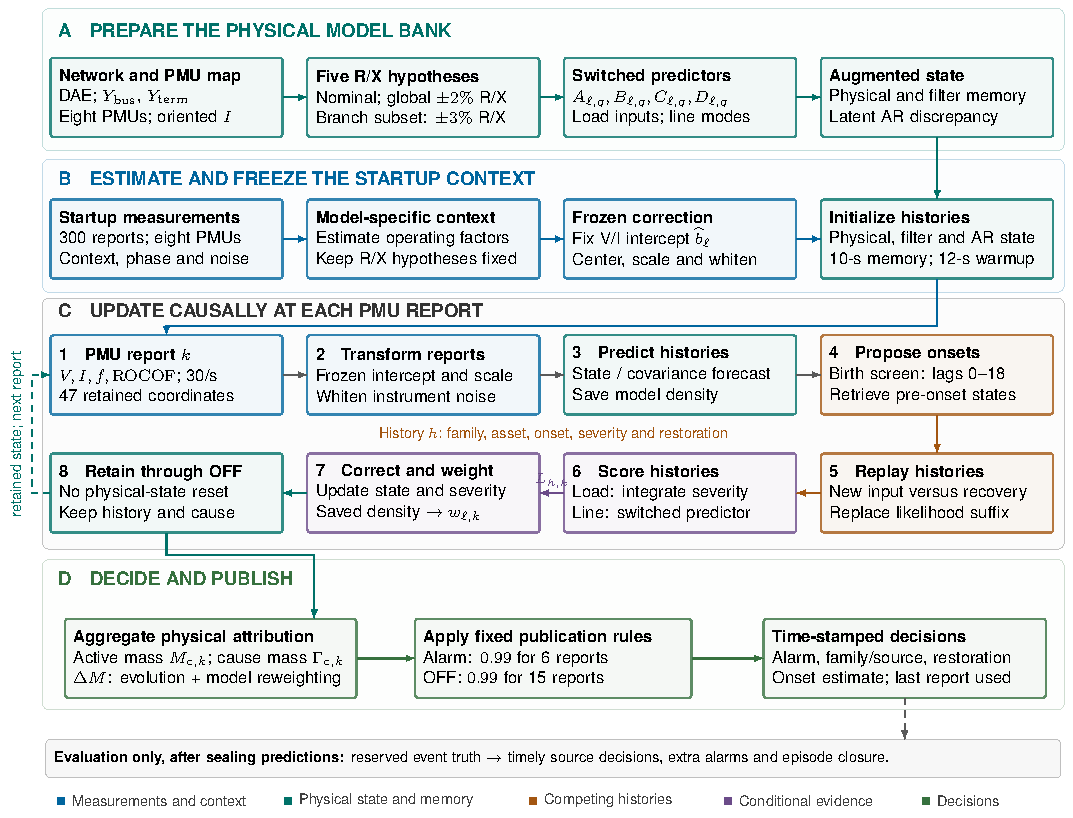
\includegraphics[width=\textwidth]{figures/generated/narrative_architecture.pdf}
\caption{Implemented physical-history attribution with its original publication policy, organized into model preparation (A), startup context (B), per-report inference (C), and publication (D). The bank predicts before state correction and saves model evidence before proposal selection. Candidate replay replaces a likelihood suffix, so each report contributes once. The feedback loop retains physical and instrumental memory through restoration. Reserved event truth is used only after predictions are sealed. The common-clock controls replace block D as specified in Section~\ref{sec:submission-checks}.}
\label{fig:joint-architecture}\end{figure*}

Physical restoration is not electrical recovery. A detector that returns
immediately to a flat reference can issue another alarm for the remaining
oscillation. Suppressing alarms throughout recovery can instead hide a real
intervention. The operating point adds another difficulty: correcting a
voltage or current offset need not correct how the network responds to a
later input.

Existing work provides strong foundations. DAE state estimators infer
unmeasured electrical states \cite{katanic2024recursive}; physical outage
detectors compare network hypotheses sequentially
\cite{chen2016quickest,rovatsos2017outage}; and simulated fault trajectories
support diagnosis from sparse PMUs \cite{warner2023highfidelity}.
Physical models, transient histories and unknown-onset searches are thus
established ingredients. A small state-reconstruction error, however, does
not by itself identify the intervention that produced the observations.

We compare physical histories rather than isolated signal features. A
history specifies an intervention, source, onset, severity and restoration.
DAE-derived predictors start from estimated past states and preserve the
state left by previous interventions. Conditional evidence integrates load
severity, accounts for instrumental memory, and updates fixed network-model
hypotheses. Separate active and cause masses keep a restored intervention
available as an explanation of the continuing response.

The paper makes three contributions within this restricted problem:
\begin{enumerate}
\item An executable attribution mechanism that makes new load/line
interventions compete with retained recovery histories. We specify its
physical predictors, evidence updates and decision rules.
\item A comparison that separates detection, correct source attribution
before restoration, extra alarms and episode closure. Nominal and uncertain
network models are evaluated alongside two fixed ExtraTrees adapters;
Chen's published detector is compared on eligible persistent line openings.
\item Adversarial tests of scope: a state-retaining physical competitor,
a classifier fitted under a grouped SIM split, and a retrospective
integrity/source replay. These tests retain failures and distinguish
simulation utility from transfer to the reference record.
\end{enumerate}

A further physical control asks whether recovery increases source separation.
It distinguishes retaining a consistent prediction from obtaining additional
information about the source; it is not a comparison of causal detectors.

On the common development cohort and publication clock, the five-model bank
obtains \SSMixTimely{}/\SSMixTotal{} timely family/source decisions with
\SSMixExtras{} extras, versus \SSSimpleTimely{}/\SSSimpleTotal{} and
\SSSimpleExtras{} for the simpler physical control. This compares complete
procedures; it does not isolate a causal effect of history retention.
\IfFileExists{generated/c01_macros.tex}{The separate
confirmatory comparison is reported below.}{The prespecified confirmatory
comparison is still running without method changes.} The claim is scoped
to the declared load/line catalog. These simulations do not establish an
all-family hackathon score, calibrated event probabilities or real-time deployment.

\section{Related Work}
\label{sec:narrative-related}

\subsection{State Estimation and Physical Source Inference}
Unknown-input and DAE estimators recover electrical states despite
incomplete models or exogenous inputs
\cite{gillijns2007input,nugroho2022dae,katanic2024recursive}. Functional
observability asks whether a requested state quantity can be recovered
\cite{fernando2010functional,montanari2022functional}. Source inference asks
which intervention can explain the trajectory. Descriptor-model
diagnosability and nuisance-profiled tests formalize this distinction
\cite{eriksson2013diagnosability,scharf1994matched}.

Physical hypotheses support outage inference from phasor angles
\cite{tate2008outage}, Bayesian inference with uncertain states
\cite{zhao2014outages}, and sequential detection under stochastic operation
\cite{chen2016quickest,rovatsos2017outage}. Anguluri \emph{et al.} recover
sparse forcing locations, inputs and an unknown initial state using group
LASSO for linear dynamics \cite{anguluri2023group}. These are precedents
for source recovery; group LASSO is not an executed comparator in our
frozen campaign. Sensor placement also affects source distinguishability
\cite{jamei2020limits,conte2023fault,yildiz2025sparse}.

\subsection{Trajectory-Based and Sequential Diagnosis}
Warner \emph{et al.} compare simulated voltage/current fault trajectories
over a moving onset window and return candidate lines
\cite{warner2023highfidelity}. Their evaluated target is short-circuit
identification before clearing; load changes are an adverse-event test.
Our target follows load changes and line openings through restoration and
successive interventions. Physical trajectory libraries, remote PMUs and
retrospective onset scanning are shared ingredients. Their procedure was
not run on our data, so no numerical superiority is inferred.

The Adaptive Matrix CuSum derives sequential identification error/delay
results under specified observation laws \cite{warner2024matrix}.
Multiple-model filtering already propagates conditional state/mode
hypotheses \cite{blom1988imm}. Our pruned history bank uses these ideas,
but its approximate covariances, proposal screen and fitted startup context
do not inherit their general guarantees. The difference tested here is how
retained recovery competes with a later intervention and affects timely
attribution and alarm burden.

\subsection{Learned Diagnosis and Physical Uncertainty}
Learned and knowledge-driven representations identify PMU disturbances and
assets \cite{pandey2020realtime,li2024knowledge,yildiz2024few}. We compare
two fixed ExtraTrees adapters from the SGSMA project. Their performance
tests transfer of those implementations, not the limits of all supervised
learning. A known physical catalog and source-excluded supervised training
also impose different information constraints.

Physical stochastic models support latent-state estimation
\cite{ensaf2023kernel,tartakovsky2023gp}, while joint DAE parameter inference
addresses uncertain generators and networks \cite{albustami2026dae}.
Our stream method uses a finite bank of constant network hypotheses.
The separate signature test examines a local event--context derivative;
it does not identify every plant parameter or replace the stream method
with an unrestricted joint estimator.

\begin{table*}[t]\centering\small
\caption{Closest inference contracts. Only Chen and the fixed ExtraTrees
adapters are executed comparators in the confirmatory stream campaign.
An untested capability is not an algorithmic impossibility.}
\label{tab:literature-capability}
\begin{tabularx}{\textwidth}{@{}lXXX@{}}\toprule
Route & Mechanism & Evaluated target & Role in this study\\\midrule
Chen / Rovatsos & Network likelihoods and sequential tests & Line outages; Rovatsos includes transients & Chen on persistent-line first decisions\\
Warner high-fidelity & Simulated V/I paths and onset search & Short-circuit line candidates & Closest trajectory precedent; no common-data run\\
Adaptive Matrix CuSum & Sequential diagnosis with error/delay analysis & One unknown distributional change & Statistical precedent; no inherited guarantee\\
DAE / stochastic-state estimation & Physical state and uncertainty models & States, unknown inputs or parameters & Components and adjacent tasks\\
Learned PMU diagnosis & Features or constrained representations & Event families and locations & Two frozen ExtraTrees references\\
Physical history bank here & Estimated-past-state paths and recovery & Successive catalog load/line events & Timely attribution, extras and restoration\\\bottomrule
\end{tabularx}\end{table*}

\section{Problem and Measurement Model}
\label{sec:narrative-problem}

At report $k$, inference uses measurements through $t_k=k/30$ to decide
whether a physical intervention occurred. Detection concerns its presence;
classification selects a physical operator; localization selects a bus or
branch. These outputs can become reliable at different times. We record
the estimated physical onset $\widehat\tau$ separately from the alarm and
diagnosis emission times.

Figure~\ref{fig:reference-event-types} introduces the broader measurement
phenomena using the known RAW0001 reference record. Faults, line changes,
generation changes and load changes alter the physical network; missing or
corrupted reports alter observation integrity. The present causal test
addresses load changes and line openings with restoration. The other panels
provide context, not additional validated event classes.

\begin{figure*}[t]\centering
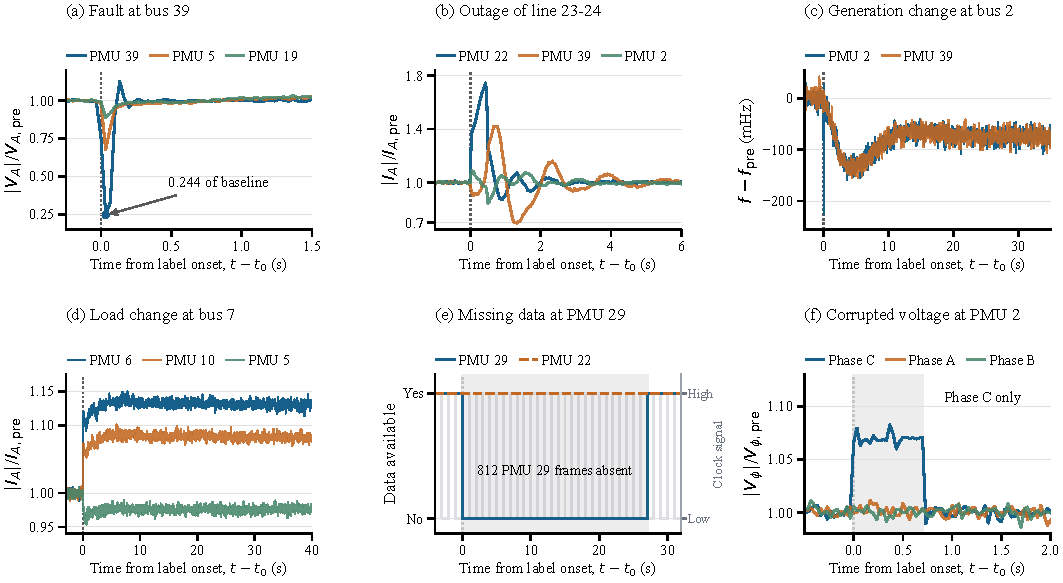
\includegraphics[width=.98\textwidth]{figures/generated/event_signatures.pdf}
\caption{Representative signatures from the archived RAW0001 reference simulation: fault, line outage, generation change, load change, missing PMU data and corrupted voltage. Alignment uses retrospective label onset for illustration; inference receives no such alignment. The gray clock in (e) is an illustrative reference, not another measured channel. Only load and line mechanisms enter the causal evaluation below. RAW0001 is known retrospective evidence, not independent field validation.}
\label{fig:reference-event-types}\end{figure*}

The network has 39 buses, but the prescribed PMU set is
\begin{equation}
 \mathcal P=\{2,5,6,10,19,22,29,39\}.
 \label{eq:narrative-pmus}
\end{equation}
Voltage is measured at each PMU bus. Current is measured at a specified branch terminal, which can differ from that bus. The causal implementation uses 47 coordinates: eight voltage magnitudes, eight voltage angles, eight current magnitudes, seven current angles, eight absolute frequencies and eight ROCOFs, at 30 reports/s. BUS39 current angle is excluded because its interpretation remains partially validated. The BUS5 current terminal retains the provisional historical 5--6 assignment. These are declared measurement assumptions, not identities inferred from classification accuracy.

The exported magnitudes are in V and A, angles in degrees, frequency in Hz
and ROCOF in Hz/s. Internal centered coordinates do not replace the
absolute frequency contract. These are reporting-rate phasor measurements;
waveform harmonics or THD are not measured by these channels.

% PROTECTED FIGURE: retain this single-column IEEE-39 diagram. See AGENTS.md.
\begin{figure}[t]\centering
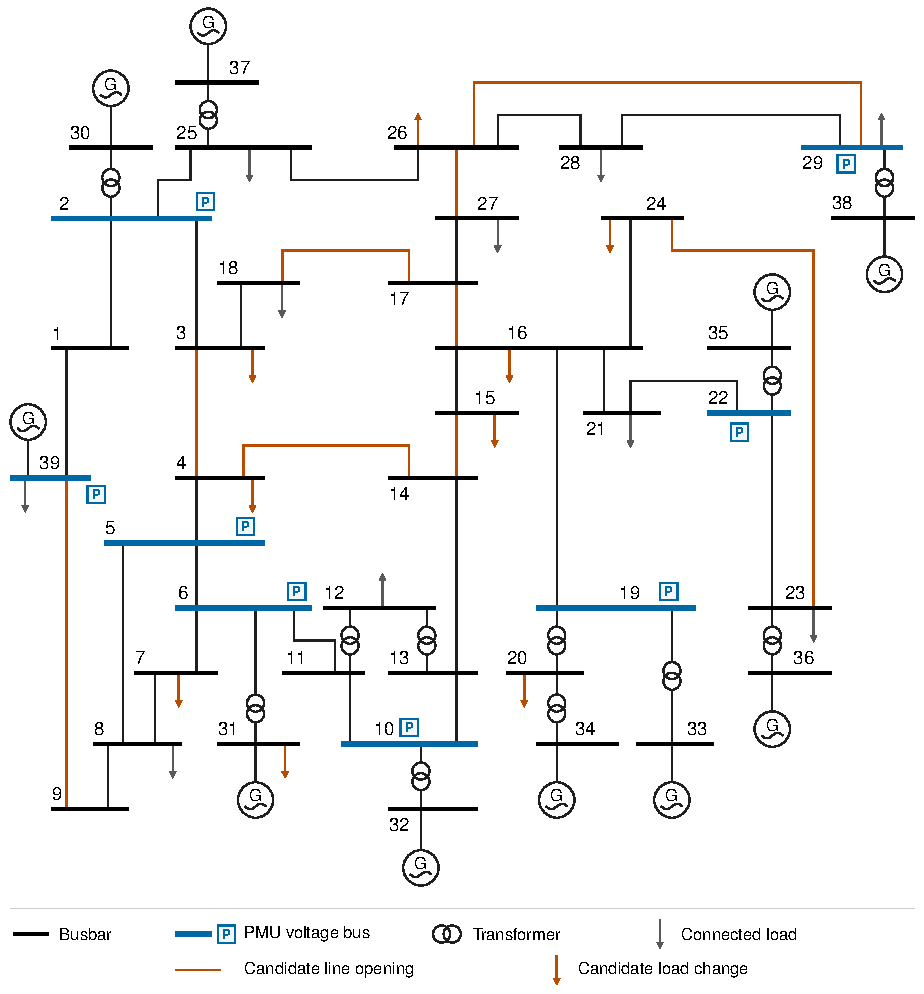
\includegraphics[width=\columnwidth]{figures/generated/narrative_topology.pdf}
\caption{IEEE 39-bus single-line diagram: 46 branches, 12 transformers and 10 generators. Blue bars and P marks locate the eight voltage PMUs. Orange branches and load arrows identify the nine line and nine load candidates; gray arrows denote other loads. Current terminals follow the separate measurement contract. All routes are orthogonal.}
\label{fig:narrative-topology}\end{figure}

The physical model is
\begin{align}
 \dot x&=f_q(x,z,u;\theta),&0&=g_q(x,z,u;\theta),\label{eq:narrative-dae}\\
 y_k&=\mathcal M_q(x_k,z_k;\theta_M)+b+\varepsilon_k.\label{eq:narrative-measurement}
\end{align}
Here $x$ contains machine and control dynamics, $z$ the algebraic network variables, $q$ the topology/intervention mode, and $\theta_M$ the measurement convention. The measurement map includes gains, phase references, orientation and the causal frequency/ROCOF estimator. A machine's rotor speed is not substituted for bus frequency.

An intervention history is $h=(e,c,\tau,a,\kappa)$: family, source, onset,
severity and restoration time, with $\kappa=\infty$ for a sustained event.
Its duration is $\kappa-\tau$ when restoration occurs. A load changes its
local P/Q setpoints; a line opening switches its branch primitive. For the
supported impulse-free switches,
\begin{equation}
 x(\tau^+)=x(\tau^-),\qquad g_{q^+}(x(\tau^-),z(\tau^+),u;\theta)=0.
 \label{eq:narrative-switch}
\end{equation}
The algebraic voltage/current response may jump even though dynamic states remain continuous. Physical restoration reverses the intervention operator. It does not return the machines to their pre-event state, so electrical recovery can continue after OFF.

\begin{table}[t]\centering\small
\caption{Scope of the executed causal component. The source is an intervention asset; it is not necessarily a measured PMU bus.}\label{tab:narrative-scope}
\begin{tabularx}{\columnwidth}{@{}lXX@{}}\toprule
Case & Physical operator & Executed claim\\\midrule
Normal & No intervention & Monitor after startup\\
Load & Local P/Q factor; optional restoration & Nine candidate buses\\
Line & Branch open; optional reclose & Nine candidate branches\\
Fault/generation & Different shunt/input/trip operators & Outside this causal test\\
Missing/bad data & Measurement-integrity mechanism & Outside C01\\
Unknown & Unresolved diagnosis & Not a new physical family\\\bottomrule
\end{tabularx}\end{table}

The generator stores event schedules and true states separately from the PMU stream. Inference receives the nominal network, permitted calibration and reports through the current time. It receives no source, switch time, true R/X realization or solver state. Initial operating context and noise scale are estimated from 300 startup reports; monitoring begins after the inherited 12-s warmup. The startup contract assumes no intervention in that prefix.

\section{Recovery-Aware Physical Attribution}
\label{sec:narrative-method}

Figure~\ref{fig:joint-architecture} describes the implemented computation.
The inference engine, archived as R11, uses a conditional history bank of
DAE-derived switched state-space predictors. The nonlinear simulator
generates observations; inference does not solve a new full nonlinear
simulation for every candidate at every report.

Physics enters the candidate dynamics, input directions and oriented
measurement map. Statistical filtering represents uncertain states and
discrepancy around those predictions. Thus the evaluated method is
model-based inference; it does not train a neural network with a physics
loss or learn a source-label classifier. A good residual fit alone is
insufficient: competing histories must also yield a timely source decision.

\subsection{Construct the Predictor From the Network}

Kirchhoff constraints and complex power connect sources to remote PMUs:
\begin{equation}
 I_{\rm bus}=Y_{\rm bus}V,\quad
 I_{{\rm term},r}=Y_{{\rm term},r}V,\quad S_i=V_i I_{{\rm bus},i}^{*}.
 \label{eq:narrative-electrical}
\end{equation}
Terminal rows retain orientation, line charging and transformer ratios.
A measured terminal current is not a nodal injection. A line opening
changes its branch primitive and terminal map; a load changes its admitted
P/Q input direction.

On a regular index-one DAE chart with a fixed angle reference,
\begin{align}
 \delta z&=-g_z^{-1}(g_x\delta x+g_u\delta u),\nonumber\\
 \delta\dot x&=A_q^{\rm red}\delta x+B_q^{\rm red}\delta u,\nonumber\\
 A_q^{\rm red}&=f_x-f_zg_z^{-1}g_x,\quad
 B_q^{\rm red}=f_u-f_zg_z^{-1}g_u.
 \label{eq:narrative-reduction}
\end{align}
For the instantaneous electrical observation map $H_q(x,z,u)$, the
corresponding output operators are
\begin{equation}
 C_q^{\rm red}=H_x-H_zg_z^{-1}g_x,\qquad
 D_q^{\rm red}=H_u-H_zg_z^{-1}g_u.
 \label{eq:electrical-output-reduction}
\end{equation}
They propagate a perturbation at an unmeasured source to the selected
voltage and oriented-current channels. Network connectivity enters through
the branch stamps in $g_q$ and $H_q$; eliminating unmeasured algebraic
variables generally produces dense reduced operators. The graph therefore
constrains the prediction without a learned graph embedding. A changed
terminal operator also contributes directly through $H_q$, not only
through the changed voltage. The implementation discretizes the admitted
switch modes and adds causal phase-history operators for frequency and
ROCOF. Inertia, controls and load law remain those of the fixed plant.

After augmenting instrumental memory, a conditional predictor has the
local form
\begin{align}
 \xi_{k+1}&=A_{\ell,q}\xi_k+b_{\ell,q}+B_{\ell,q}a+w_k,\nonumber\\
 r_k&=C_{\ell,q}\xi_k+d_{\ell,q}+D_{\ell,q}a+v_k.
 \label{eq:implemented-predictor}
\end{align}
Here $r_k$ contains reference-corrected, scaled and instrument-whitened PMU coordinates, $\ell$ is a fixed
network hypothesis, and $\xi_k$ contains physical deviation states, phase
history and predicted measurement-filter memory. Observed colored-instrument
filters whiten measurements; their corresponding predictor memory is
deterministic. Additional latent AR states represent persistent discrepancy,
with preset quiet/load/line/recovery covariance and drift regimes. This
statistical discrepancy model is distinct from the plant equations.
$v_k$ denotes the remaining innovation. A load has scalar severity within
its specified P/Q direction. A line uses a switched operator rather than
a fictitious load-amplitude fit. States from different equilibria are not
interpreted as an absolute rotor-state mixture.

\subsection{Estimate Context From the Startup Prefix}

Each network hypothesis uses the same 300 startup reports to estimate
operating factors, reference phase and noise scale. Voltage/current
coordinates receive a constant discrepancy correction,
\begin{equation}
 \widehat b_\ell=\overline y_{0:299}-y_\ell^{\rm ref},
 \qquad b_{\ell,k}=\widehat b_\ell\quad(k\ge300).
 \label{eq:continuous-intercept}
\end{equation}
Angular differences respect wrapping and the common reference. Frequency
and ROCOF use empirical prefix centers. The correction remains fixed so it
cannot track a later load step and subtract its signature. This estimates
an observation discrepancy, not the true impedances. Prefix estimates
enter by substitution rather than through a full joint parameter posterior.

\subsection{Compare Unknown-Onset Histories}

The method retains ten seconds of past conditional states. Its frozen
birth screen searches lags of 0--18 reports and proposes selected onsets;
it does not enumerate every onset in the 300-report history.
Each history specifies family, asset, onset,
restoration mode and severity. It starts from the stored conditional state
before its proposed onset. That state already contains any ongoing
recovery; an alarm does not reset the predictor to equilibrium.

For a retained load history, conditional Gaussian filtering yields a
residual $e$, severity response $s$ and covariance $S$. Unknown severity
has a truncated-Gaussian distribution inherited from previous reports:
\begin{equation}
 L_{h,k}=\int_l^u \mathcal N(e;sa,S)
             \operatorname{TN}_{[l,u]}(a;\mu,v)\,da.
 \label{eq:narrative-evidence}
\end{equation}
With $\Phi$ denoting the standard normal CDF, define
\begin{align}
 v'&=(v^{-1}+s^\top S^{-1}s)^{-1},\nonumber\\
 \mu'&=v'(\mu/v+s^\top S^{-1}e),\nonumber\\
 Z(\mu,v)&=\Phi((u-\mu)/\sqrt v)-\Phi((l-\mu)/\sqrt v).
\end{align}
The implemented local integral follows by completing the square:
\begin{align}
 \log L_{h,k}&=\log\mathcal N(e;0,S)+\tfrac12\log(v'/v)\nonumber\\
 &\quad+\tfrac12(\mu'^2/v'-\mu^2/v)
       +\log\frac{Z(\mu',v')}{Z(\mu,v)}.
 \label{eq:amplitude-evidence-main}
\end{align}
These standard identities are exact for the stated local conditional
model. Adaptive proposals, pruning and covariance approximations make the
complete bank approximate.

The conditional state mean is represented as $m_h+d_h a$. To make the
filtering approximation explicit, let $T_o,J_o,g_o,u_o,j_o,v_o$ denote the
archived one-report transition and observation operators for switch $o$.
The code forms $e=r_k-J_o m_h-j_o$ and $s=J_o d_h+v_o$. With the shared
covariance $P_\rho$ for the current discrepancy regime $\rho$,
\begin{align}
 S_o&=R+J_oP_\rho J_o^\top,&
 K_o&=T_oP_\rho J_o^\top S_o^{-1},\nonumber\\
 m_h^+&=T_o m_h+g_o+K_o e,&
 d_h^+&=T_o d_h+u_o-K_o s.
 \label{eq:implemented-conditional-correction}
\end{align}
The amplitude distribution is updated by the same integral above. The
regime covariances are obtained from nominal-operator Riccati equations;
R11 does not propagate an independent exact covariance for every switched
history. At episode closure, it retains the mixture mean of the augmented
state and records the omitted between-history spread. Thus state continuity
and conditional Bayesian amplitude integration are implemented, while a
fully Bayesian posterior over states, context and all histories is not.

The rolling screen proposes histories; it is not another independent
observation. Replaying a suffix replaces its original no-new-event suffix
likelihood. The sequential update therefore counts each report once,
rather than repeatedly accumulating overlapping ten-second windows.

\begin{figure*}[t]\centering
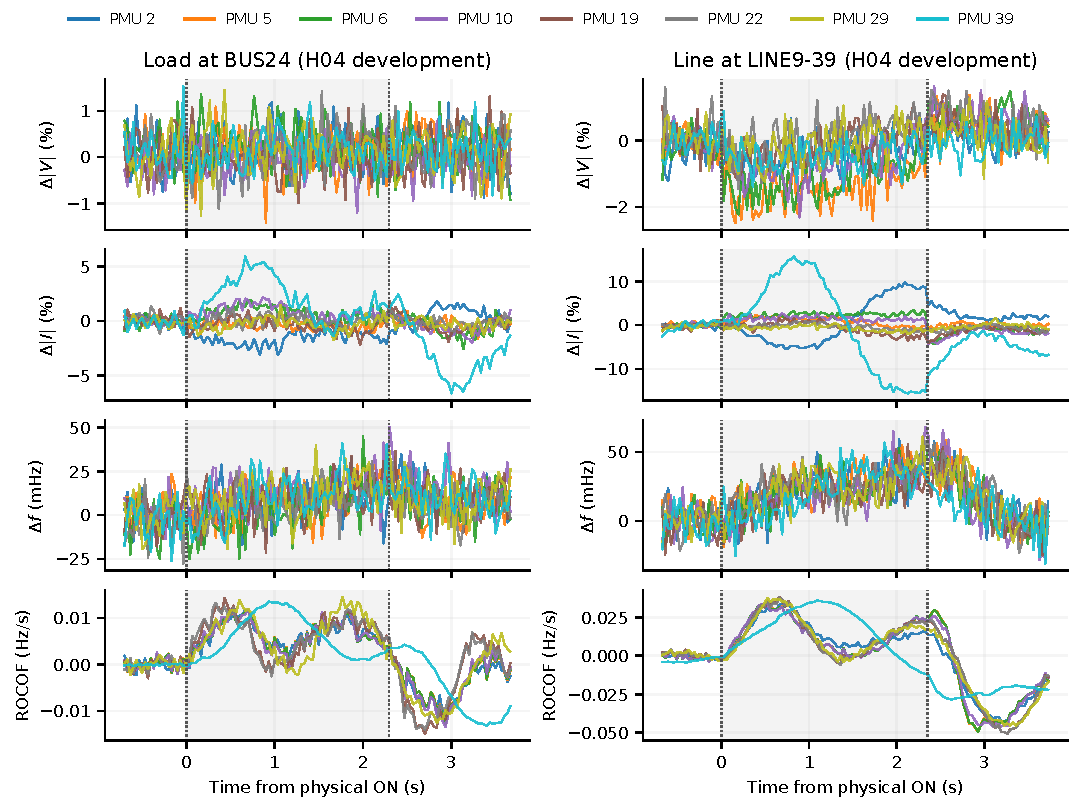
\includegraphics[width=.96\textwidth]{figures/generated/narrative_signals.pdf}
\caption{Simulated observations supplied to inference. One fixed development parent provides a load and a line example at all eight PMUs. Shading marks physical ON--OFF for evaluation only. Magnitude changes use the local pre-event center; frequency is centered for display while its exported channel remains absolute Hz. Source, severity and operating context affect the curves, so they are not universal class templates.}
\label{fig:narrative-signals}\end{figure*}

\subsection{Represent Fixed Network Uncertainty}

The bank contains nominal, global $\pm2\%$, and selected-branch $\pm3\%$
paired R/X hypotheses. Parameters stay constant within a hypothesis. Its
outer weight uses a predictive density formed before the current-report
state update and proposal selection:
\begin{equation}
 w_{\ell,k}=\frac{w_{\ell,k-1}p_\ell(y_k\mid\mathcal F_{k-1},\widehat b_\ell)}
 {\sum_jw_{j,k-1}p_j(y_k\mid\mathcal F_{k-1},\widehat b_j)}.
 \label{eq:continuous-weights}
\end{equation}
Startup-fitting reports are not scored again as independent model-selection
evidence. The mixture covers a finite set of network alternatives rather
than identifying a continuous impedance posterior.

\subsection{Keep Recovery as a Competing Physical Explanation}

Restoring an input or topology at $\kappa$ does not restore the pre-event
state: $x(\kappa^+)=x(\kappa^-)$. On a regular local post-restoration chart,
the difference from a same-context no-new-intervention trajectory obeys
\begin{align}
 \delta x_h(t)&\simeq\Phi_0(t,\kappa)\delta x_h(\kappa),\nonumber\\
 \delta y_h^{\rm net}(t)&\simeq C_0(t)\Phi_0(t,\kappa)\delta x_h(\kappa),
 \quad t>\kappa.
 \label{eq:recovery-response}
\end{align}
Here $y^{\rm net}$ denotes voltage/current coordinates before the instrument map.
Instrumental memory is retained as well. This local interpretation of known
dynamics explains why the reference after OFF is a trajectory, not a zero
residual; it is not a new propagation theorem.

For conditional history mass $\pi_{\ell,h,k}$, define active and
originating-cause masses for an admissible family/source cell $c$:
\begin{align}
 M_{c,k}&=\sum_\ell w_{\ell,k}\sum_{h:c(h)=c}
       \pi_{\ell,h,k}\,\mathbf1\{h\text{ active at }k\},\nonumber\\
 \Gamma_{c,k}&=\sum_\ell w_{\ell,k}\sum_{h:c(h)=c}\pi_{\ell,h,k}.
 \label{eq:active-cause-masses}
\end{align}
A retained history can stop being active while its cause still explains
recovery. Later interventions compete with those histories. The
implementation stores 18 admissible cells, not every family at every bus.
After confirmed episode closure, explicit histories are compressed into
the retained state mean. Cause masses describe the current bank, not a
permanent ledger of all past interventions.

Writing the conditional active mass as $M_{\ell,c,k}$ yields
\begin{align}
 \Delta M_{c,k}&=\sum_\ell w_{\ell,k}
               (M_{\ell,c,k}-M_{\ell,c,k-1})\nonumber\\
 &\quad+\sum_\ell(w_{\ell,k}-w_{\ell,k-1})M_{\ell,c,k-1}.
 \label{eq:continuous-delta}
\end{align}
The terms distinguish within-model evolution from model reweighting.
This accounting identity aids interpretation, without constituting a new
tensor factorization. The masses are approximate attribution weights;
probability calibration and globally optimal filtering are not established.

\subsection{Emit Separate Detection, Diagnosis and Restoration Messages}

The fixed publication rules require active mass 0.99 for six reports to
confirm an alarm, and restoration mass 0.99 for 15 reports to confirm OFF.
The archived source/line confirmation and episode-replacement rules
determine the public diagnosis. Every message records emission time and
the last report used. A diagnosis can be correct eventually but too late
to precede physical OFF.

The nominal comparator uses the same nominal conditional model with its
own fixed publication path. Comparing nominal and mixture evaluates two
complete configured procedures; it does not isolate the outer network bank
from publication decisions. The admission-rule ablation tests a different publication
decision; it is not a pure recovery-memory ablation.

The per-report birth and restoration hazards are
$1-\exp[-(1/60)/30]$ and $1-\exp[-(1/30)/30]$.
Birth mass is split equally between load and line families, then uniformly
among sources within each family. Load severity has a zero-mean Gaussian
prior with standard deviation 0.15, truncated to $[-0.2,0.2]$ and integrated
over four intervals with boundaries $-0.2,-0.1,0,0.1,0.2$.
After three reports, eligible active histories can produce OFF children
at either half-report position while inheriting state and severity.
After likelihood normalization, the beam retains the 96 highest-weight
recent histories, 64 older histories and at least one per occupied source;
their union is renormalized and discarded mass is recorded.
The reproducibility archive maps these operations to the frozen
\texttt{transitions}, \texttt{process}, and
\texttt{predictive\_log\_density} routines and preserves the complete
publication configuration.

\subsection{Per-Report Algorithm and Computational Boundary}

\noindent\textbf{Algorithm 1: causal physical-history attribution.}
The inputs are the nominal model, fixed method configuration and successive
PMU reports. Reserved event truth never enters these steps.
\begin{enumerate}
\item Estimate operating context, common reference and noise scale from the
startup prefix. Initialize conditional states and retain the eligible past
states needed by retrospective proposals.
\item At report $k$, apply the frozen centering, scaling and instrumental
transformation. Propagate each retained physical/recovery history and its
conditional uncertainty to predict this report. Compute and save the outer
model predictive density before current-report screening and state correction.
\item Apply the frozen short-lag birth screen using retained past states.
A proposed history starts before its selected onset; replay
replaces the corresponding likelihood suffix rather than adding it twice.
\item Score candidate histories and replayed suffixes before correcting
their states with the reports being scored. Integrate the allowed load severity and apply
the archived switched operator for a line hypothesis.
\item Correct the conditional states and severity distributions; update
network weights and the retained history bank using the fixed rules.
Preserve dynamic state and originating cause through restoration.
\item Aggregate active mass $M$, cause mass $\Gamma$ and $\Delta M$.
Apply the fixed alarm, diagnosis and OFF-publication rules. Store emission
time, estimated onset, family/source and the last report used.
\end{enumerate}
The nonlinear simulator constructs observations; this algorithm propagates
local switched predictors. The input grid is 30 reports/s. Causality
concerns report availability; acquisition throughput, computation time
and the electrical history needed for a decision are separate quantities.
Wall-clock real-time operation has not been established.

\FloatBarrier
\section{Experimental Design}
\label{sec:narrative-protocol}

The primary experiment asks whether the causal bank can attribute successive load/line interventions without confusing recovery with a new event. Development, independent evaluation and an auxiliary source-resolution experiment answer different questions and retain separate denominators.

\begin{table*}[t]\centering\small
\caption{Experimental populations and their purposes. Conditions and noise realizations repeat a physical parent rather than creating independent trajectories.}\label{tab:narrative-evidence}
\begin{tabularx}{\textwidth}{@{}lXXX@{}}\toprule
Population & Configuration & Main outcome & Interpretation\\\midrule
Continuous development & Three event parents, six interventions each; one normal parent; three network conditions & Timely family/source, extras and restoration & Open development evidence, not independent confirmation\\
Independent continuous evaluation & 18 event parents, six interventions each; 12 normal parents; three network conditions and two noise scales & Paired attribution, false alarms, delays and failures & Prespecified comparison of unchanged methods\\
Persistent-line evaluation & Nine lines, three parent repetitions; same network/noise strata & First stopping decision, source and censoring & Eligible comparison with published line-outage QCD\\
\IfFileExists{generated/ei_x02_macros.tex}{Signature component test & \EIDictionaryCases{} dictionary and \EITestPhysical{} test trajectories; four loads; three common noise seeds & Nominal, reference correction and mixed-signature correction & Known ON/OFF and family; separate from causal accuracy\\}{}
Recovery geometry control & 38 trajectories; four recovery histories and 12 correlated source-pair comparisons & Separation with known history and one uncertain severity direction & Supplied prior trajectory, onset, family and pair; not R11 performance\\
\bottomrule
\end{tabularx}\end{table*}

The simulator is the IEEE-39 Julia/PowerDynamics research candidate F01. Each physical parent is integrated continuously, preserving differential states through ON/OFF. Its PMU reporting grid is separate from solver steps: a 120-s record contains 3601 reports per PMU and a 600-s normal record contains 18001, including endpoints. At a switch-aligned report the export uses the post-switch algebraic value. Measurement references, load law and stochastic instrument parameters are fixed across events. RAW0001 supplied retrospective calibration context, not independent test data.

H03 and H04 each contain three event parents with six successive load/line interventions and one normal parent, all 80 s long. Schedules are paired across nominal, in-bank R/X and mixed out-of-bank R/X conditions. Each campaign therefore has 18 unique interventions and 54 event realizations. Both campaigns are now development evidence. No interval or generalization claim treats those 54 realizations as independent events.

R11 and its nominal version are frozen co-references. Both ExtraTrees artifacts and their causal preprocessing/publication adapters are frozen as well; neither is retrained on H04 or C01. They receive the same 30-fps observations. This is a comparison of those operational implementations on the stated contract, not a rerun of the hackathon leaderboard.

The published physical comparator is Chen \emph{et al.}'s persistent single-line quickest-change detector \cite{chen2016quickest}. Its reduced-network covariance is marginalized to the observed PMU subset after inversion. Parallel CUSUM statistics stop at the first threshold crossing and select a line. Our declared F01 adapter uses nonoverlapping angle increments at 15 Hz, a startup-only scale/drift estimate and the fixed nominal line catalog. Its white-injection/DC assumptions do not describe all F01 instrumental effects. We preserve both matched-law implementation checks and F01 mismatch failures; no ARL guarantee is transferred to colored noise.

The eligible common test for Chen is one persistent line opening or a normal record. Its output has no load family or restoration operator. The independent campaign, C01, therefore separates continuous load/line episodes from persistent-line first-stop decisions. Early stops, wrong sources, omissions and horizon censoring remain visible.

For continuous events, an alarm is associated temporally before predicted family/source is inspected. The first unmatched alarm after ON is eligible up to the next ON, with the inherited 30-s cap. A timely joint decision requires the correct family and asset emitted before true OFF. Unmatched alarms are extras; false restorations and open episodes are reported separately. These definitions prevent an eventual correct answer from hiding a late diagnosis.

C01 specifies 18 continuous parents, 27 persistent-line parents and 12 normal parents, with three R/X conditions and instrumental-noise scales of one and two. The 171 intended physical trajectories yield 342 observed records. Conditions represent nominal parameters, perturbations represented in the bank and mixed perturbations outside it. Solver and inference failures remain in the intended denominators. Comparisons use 10,000 paired parent-cluster resamples; repeated conditions/noise do not count as independent parents. Predictions are fixed before the evaluator opens reserved truth.

Logical decision delay is measured on report timestamps. Wall-clock cost is recorded separately with hardware, process concurrency and one-thread BLAS settings; parallel execution of independent records does not make a within-record inference method real-time. \IfFileExists{generated/c01_macros.tex}{The completed independent results follow the development examples.}{The independent evaluation is in progress. The following section reports completed development results only.}

\FloatBarrier
\section{Continuous-Stream Results}
\label{sec:narrative-results}

\subsection{Timely Attribution and Extra Alarms Measure Different Outcomes}

This section uses each frozen method's original publication policy.
The common-clock physical control in Section~\ref{sec:submission-checks}
re-publishes the same history-bank outputs under a different declared rule;
its counts are a separate endpoint. The ExtraTrees rows here are the
archived R09 references, distinct from the newly fitted S01 classifier.\AIDraftingCredit{}

\begin{table}[t]\centering\small
\caption{H04 with the original publication policies. ExtraTrees rows are archived R09 comparators. Load and line columns require the correct family and source emitted before OFF. The 54 realizations repeat 18 interventions across three R/X conditions; they are not 54 independent trials. Normal exposure is only 204 s per method.}
\label{tab:narrative-results}
\setlength{\tabcolsep}{3pt}\begin{tabular}{lrrrr}\toprule
Method & \shortstack{Load\\timely} & \shortstack{Line\\timely} & Extras & \shortstack{Normal\\alarms}\\\midrule
Physical (5 models) & 26/27 & 27/27 & 4 & 0\\
Physical nominal & 27/27 & 27/27 & 7 & 0\\
Archived ET ref. & 0/27 & 27/27 & 3 & 0\\
Archived ET short & 0/27 & 27/27 & 3 & 0\\
Onset witness & 25/27 & 27/27 & 0 & 0\\
\bottomrule\end{tabular}\end{table}


In H04, both ExtraTrees adapters and both physical references identify all tested lines in time (Table~\ref{tab:narrative-results}). The difference is in loads: the five-model bank obtains \NarMixLoadTimely{}/\NarMixLoadTotal{} timely decisions, nominal \NarNomLoadTimely{}/\NarNomLoadTotal{}, and these ExtraTrees adapters \NarETLoadTimely{}/\NarETLoadTotal{}. This tests transfer of the frozen adapters; it neither rules out supervised load detection nor reproduces the historical multi-class hackathon score.

The five-model bank detects and eventually attributes \NarMixJoint{}/\NarMixEvents{} realizations, but only \ContMixTimely{} diagnoses precede physical OFF. Nominal has \ContNomTimely{} timely diagnoses, with \ContNomExtras{} extras versus \ContMixExtras{}. Detection, eventual attribution and timely attribution therefore give different answers. The configured five-model procedure yields one fewer timely diagnosis and three fewer extra alarms than nominal; this comparison does not isolate model uncertainty.

\subsection{Recovery and a New Event Must Remain Competing Explanations}

Figure~\ref{fig:narrative-rolling} shows what the counts omit. The physical state continues evolving after OFF. Retained cause/recovery histories explain that trajectory without resetting the network; a later source must compete against both no-new-event recovery and other interventions.



The out-of-bank BUS31 case shows a remaining timing failure: the source is recovered eventually but too late. The network mixture changes how much mass is assigned to that source, and \eqref{eq:continuous-delta} separates that revision from within-model evidence. This decomposition distinguishes changing within-model evidence from changing network weights; it is an interpretation of the delayed decision.

\begin{figure}[!htbp]\centering
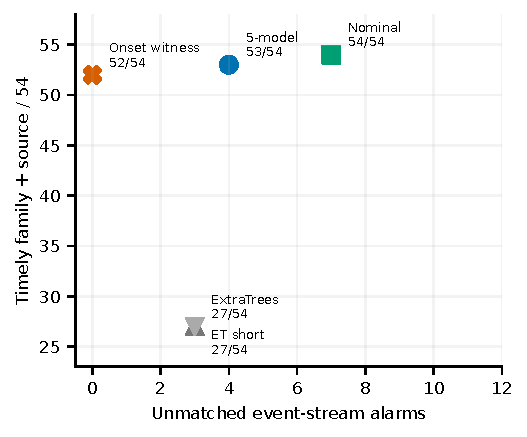
\includegraphics[width=\columnwidth]{figures/generated/narrative_tradeoff.pdf}
\caption{The decision that an accuracy-only table hides. H04 development outcomes trade timely attribution against unmatched event-stream alarms. The onset-witness ablation removes all extras but loses a real BUS16 intervention; it is retained as negative evidence. Labels use 54 paired realizations of 18 interventions and do not imply 54 independent trials.}
\label{fig:narrative-tradeoff}\end{figure}

The onset-witness ablation obtains zero extras but only \ContAdmissionTimely{}/\ContAdmissionTotal{} timely attributions: weak early evidence rejects a real BUS16 load. It inherits the physical states and masses, so suppressing the alarm does not repair the underlying explanation. This negative experiment leaves R11 and nominal frozen for C01.

\begin{figure*}[p]\centering
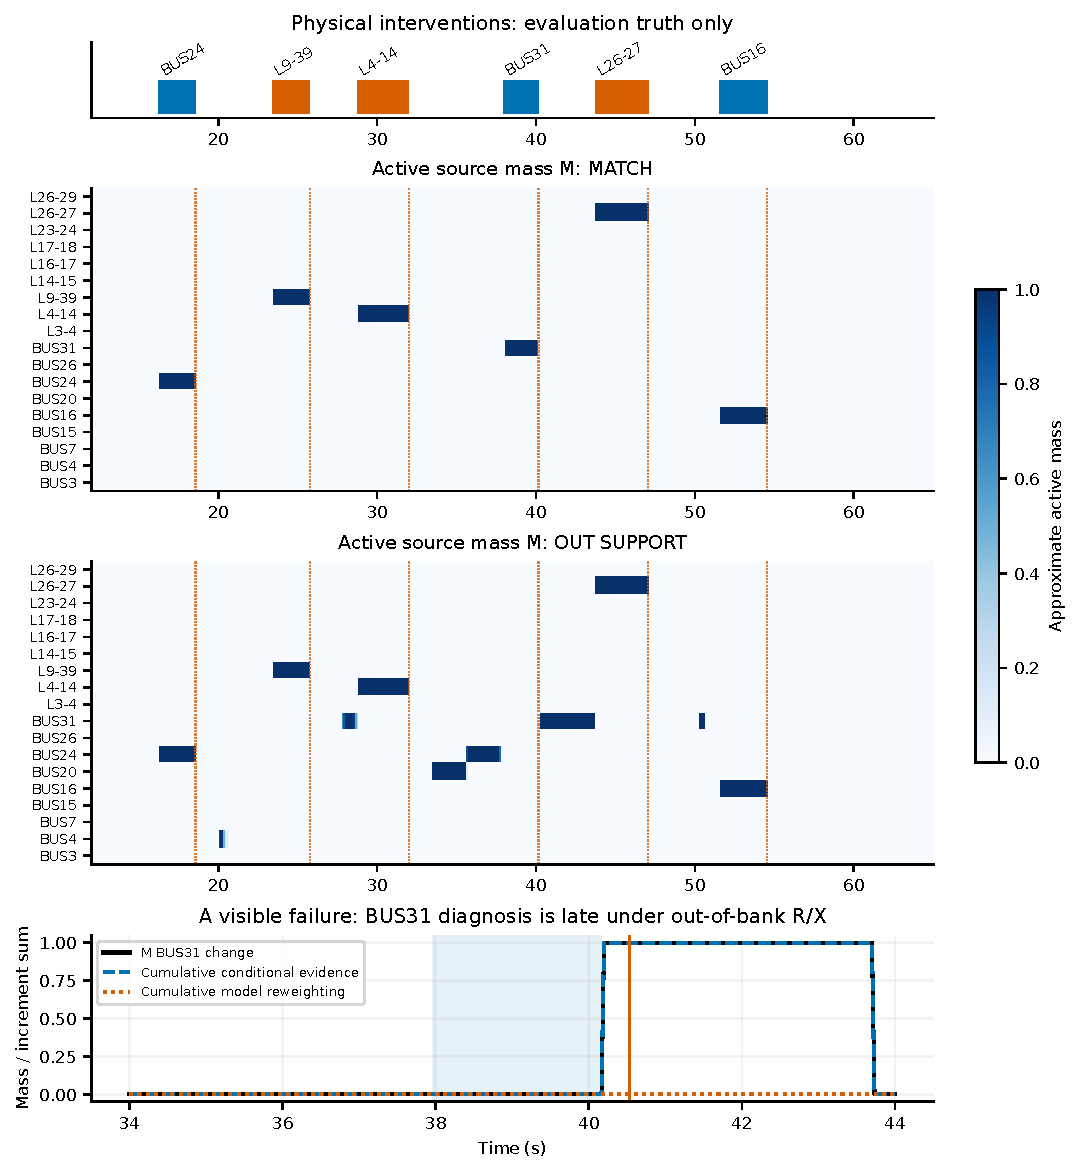
\includegraphics[width=.95\textwidth]{figures/generated/narrative_rolling.pdf}
\caption{From a continuous sequence to source attribution. Top: reserved physical ON--OFF intervals in development parent H002. Middle: active masses for nominal-network observations (MATCH) and mixed R/X changes outside the bank (OUT SUPPORT). Orange dotted lines mark true OFF for evaluation only. Bottom: BUS31 in the latter record; the cumulative terms of $\Delta M$, rebased at 34 s, sum to the change in active mass. Diagnosis arrives after OFF. The figure shows an eventual correct source that fails timely attribution; the color scale represents approximate mass, not calibrated probability.}
\label{fig:narrative-rolling}\end{figure*}

\FloatBarrier
\IfFileExists{sections/08c_c01_confirmatory.tex}{\input{sections/08c_c01_confirmatory}\FloatBarrier}{}
\IfFileExists{generated/ei_x02_macros.tex}{\section{Operating-Point Signature Experiment}
\label{sec:ei-x02}

\subsection{Reference Correction and Response Correction}
The stream bank already builds local predictors at estimated operating
points. A separate experiment tests why changing a reference alone may be
insufficient. It compares three response approximations with identical
observations, channels, timing, amplitude prior and inference horizon.
It is a controlled test of a mixed derivative, not another version of R11.

Let $\eta$ denote a scalar operating change and $a$ the signed load factor.
Central differences of complete nonlinear DAE trajectories give
\begin{align}
 D_i(\eta)&\simeq\frac{y_i(\eta,h)-y_i(\eta,-h)}{2h},\nonumber\\
 E_i&\simeq\frac{D_i(d)-D_i(-d)}{2d}.
 \label{eq:ei-mixed-response}
\end{align}
The event follows the same ON/OFF schedule in every derivative trajectory.
The fixed $Q_i^0$ is the coefficient of $a^2$, obtained from the centered
second difference divided by $2h^2$. After removing the frozen common
angle drift, the three predicted histories are
\begin{align}
 \mu_i^{\rm N}(a)&=y_0+aD_i^0+a^2Q_i^0,\nonumber\\
 \mu_i^{\rm R}(a)&=\mu_i^{\rm N}(a)+\widehat b,\nonumber\\
 \mu_i^{\rm E}(a)&=\mu_i^{\rm R}(a)+a\widehat\eta E_i.
 \label{eq:ei-three-predictions}
\end{align}
Both corrected variants use exactly the same prefix offset $\widehat b$.
This comparator corrects the measured PMU reference; it is not the separate
nonlinear AC hidden-state reconstruction algorithm in the historical study.
Only the last changes the event signature. The first two consequently
have identical incremental response models even when their absolute fits
differ. Context $\widehat\eta$ is estimated by generalized least squares
from the pre-event PMUs and the nominal context direction. No test context,
source or severity enters inference.

\begin{figure*}[t]\centering
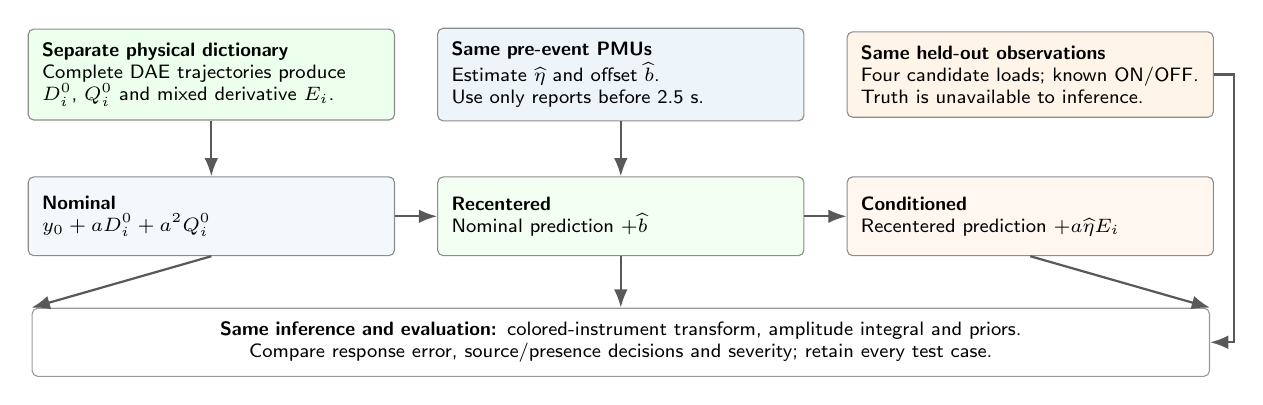
\begin{tikzpicture}[font=\sffamily\scriptsize,>=Latex,
 b/.style={draw=black!45,rounded corners=2pt,align=left,text width=4.3cm,minimum height=1.0cm,inner sep=5pt},
 a/.style={->,draw=black!65,thick}]
\node[b,fill=accessblue!7] (prefix) at (5.2,0) {\textbf{Same pre-event PMUs}\\Estimate $\widehat\eta$ and offset $\widehat b$.\\Use only reports before 2.5 s.};
\node[b,fill=green!7] (dict) at (0,0) {\textbf{Separate physical dictionary}\\Complete DAE trajectories produce\\$D_i^0$, $Q_i^0$ and mixed derivative $E_i$.};
\node[b,fill=orange!9] (data) at (10.4,0) {\textbf{Same held-out observations}\\Four candidate loads; known ON/OFF.\\Truth is unavailable to inference.};
\node[b,fill=accessblue!5] (nom) at (0,-1.8) {\textbf{Nominal}\\$y_0+aD_i^0+a^2Q_i^0$};
\node[b,fill=green!5] (recent) at (5.2,-1.8) {\textbf{Recentered}\\Nominal prediction $+\widehat b$};
\node[b,fill=orange!6] (cond) at (10.4,-1.8) {\textbf{Conditioned}\\Recentered prediction $+a\widehat\eta E_i$};
\node[draw=black!40,rounded corners=2pt,text width=14.6cm,align=center,inner sep=5pt] (out) at (5.2,-3.4) {\textbf{Same inference and evaluation:} colored-instrument transform, amplitude integral and priors.\\Compare response error, source/presence decisions and severity; retain every test case.};
\draw[a] (dict)--(nom);\draw[a] (prefix)--(recent);
\draw[a] (nom)--(recent);\draw[a] (recent)--(cond);
\draw[a] (data.east)--++(.25,0)|-(out.east);
\draw[a] (nom.south)--(out.north west);\draw[a] (recent)--(out);\draw[a] (cond.south)--(out.north east);
\end{tikzpicture}
\caption{Executed signature ablation, separate from the stream algorithm
in Fig.~\ref{fig:joint-architecture}. The three variants share the data
and decision calculation; only reference and event-response terms differ.}
\label{fig:ei-architecture}\end{figure*}


\subsection{Test Cases and Decision Contract}
The frozen F01 plant supplies all trajectories. The scalar $\eta$ scales
PQ operating injections and active PV dispatch; feasible initialization
can change permitted operating setpoints, but not machine constants,
line impedances, ZIP fractions or the PMU model. Central event/context
steps are 0.005 and 0.01, with step-halving checks. Dictionary construction
uses \EIDictionaryCases{} trajectories. The test contains \EITestPhysical{}
physical cases: \EIEventPhysical{} load interventions and \EINormalPhysical{}
controls at operating changes $-3\%,-2\%,0,+2\%,+3\%$. Each load changes
P/Q together by $\pm0.1\%$ or $\pm1\%$ at BUS3, BUS7, BUS16 or BUS24.
None belongs to the prescribed voltage-measurement PMU set; the separate
oriented current-terminal assignments remain fixed.

Each case is one ten-second integration, with ON at 3 s, OFF at 6 s and
no state reset. The context fit ends at 2.5 s. Three frozen instrumental
noise seeds produce \EIObserved{} paired records. The nonlinear PMU
frequency/ROCOF operator runs before its archived instrumental noise is
added. Both corrected methods retain the same measured prefix, so an
advantage cannot arise from supplying one method a better initial reference.\AIDraftingCredit{}

This experiment supplies the load family and ON/OFF times. It estimates
source and continuous severity using the same bounded Gaussian prior and
amplitude-integrated likelihood in all three variants. The no-event
hypothesis is retained. The fixed colored-instrument transform is common;
plug-in prefix estimates and clipped noise still limit probability
calibration. Thus these decisions are not unknown-onset detector scores
and normal-window decisions are not continuous false-alarm rates.

\subsection{Response Error and Source Decisions}
% Transposed from the generated X02 table, without changing values.
\begin{table}[t]\centering\footnotesize\setlength{\tabcolsep}{3pt}
\caption{Controlled known-onset load test. Response error uses 80 physical cases; joint and source-only correctness use 240 noisy event records. Severity error is evaluated at the generating source. The 15 normal windows are not normal-hours exposure.}
\label{tab:ei-results}
\begin{tabular}{lrrr}\toprule
Measure & Nominal & Recentered & Conditioned\\\midrule
Response error (\%) & 1.25 & 1.25 & 0.0561\\
Joint correct & 114/240 & 240/240 & 240/240\\
Source-only correct & 114/240 & 240/240 & 240/240\\
Normal selections & 12/15 & 0/15 & 0/15\\
Severity error (\%) & 3.45 & 1.2 & 0.329\\
\bottomrule\end{tabular}\end{table}

Relative to recentering alone, the mixed term reduces mean incremental response error: the paired difference is -1.15 percentage points (95\% interval [-1.31, -1]). The corresponding joint-decision difference is 0 percentage points ([0, 0]), which does not establish a directional improvement in joint source decisions. The recentered and conditioned source decisions are already at the test ceiling. Median absolute relative severity error, evaluated at the generating source, changes from 1.2\% to 0.329\%. Its mean paired change is -0.738 percentage points ([-0.898, -0.582]). Both variants select the correct source in every tested event record, so this severity comparison does not discard source errors. Their source masses numerically saturate at one; zero recorded log-loss is not evidence of calibrated uncertainty.


The gain is not uniform across all comparisons: at the nominal operating
point, estimating an unnecessary reference/context can worsen severity
relative to keeping the correct fixed reference. Figure~\ref{fig:ei-comparison}
retains that case rather than reporting only shifted operation.

The derivative stability checks change $E_i$ by
\EIContextFDLow{}--\EIContextFDHigh{}\% when the
context step is halved. Halving the event step in the two checked directions
changes it by at most \EIEventFDHigh{}\%. These are local numerical checks, not a
global smoothness or identifiability certificate.
Percentages of event severity refer to the P/Q input factors; actual load
power also responds to voltage under the frozen impedance law.

\begin{figure*}[t]\centering
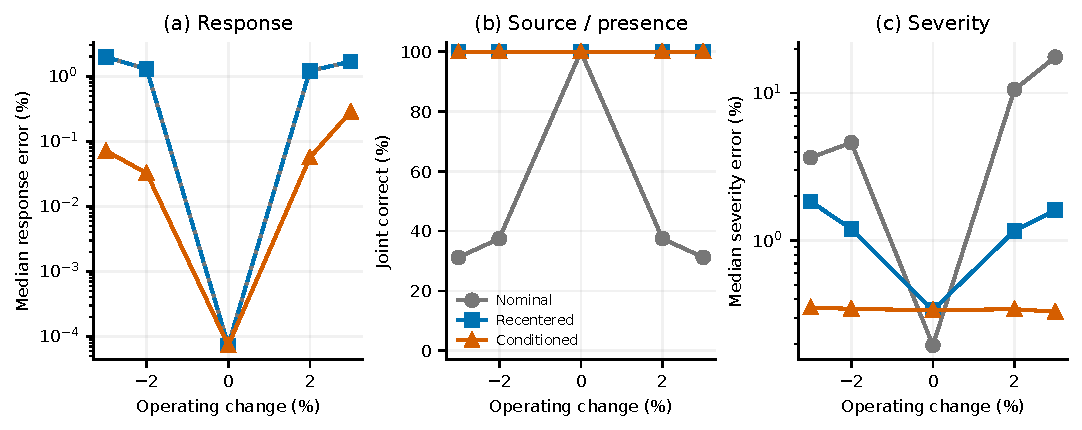
\includegraphics[width=.96\textwidth]{figures/generated/ei_x02_comparison.pdf}
\caption{Separate effects of recentering and conditioning. (a) Incremental
response error in the fixed physical test cases, evaluated at the generating
source and severity to isolate approximation error. (b) Correct source
and presence decisions on noisy observations, after marginalizing severity.
(c) Relative severity error evaluated at the generating source.
The panels measure different outcomes. Noise realizations repeat
physical cases and are not counted as additional independent trajectories.
Nominal and recentered incremental predictions coincide.}
\label{fig:ei-comparison}\end{figure*}

\begin{figure*}[t]\centering
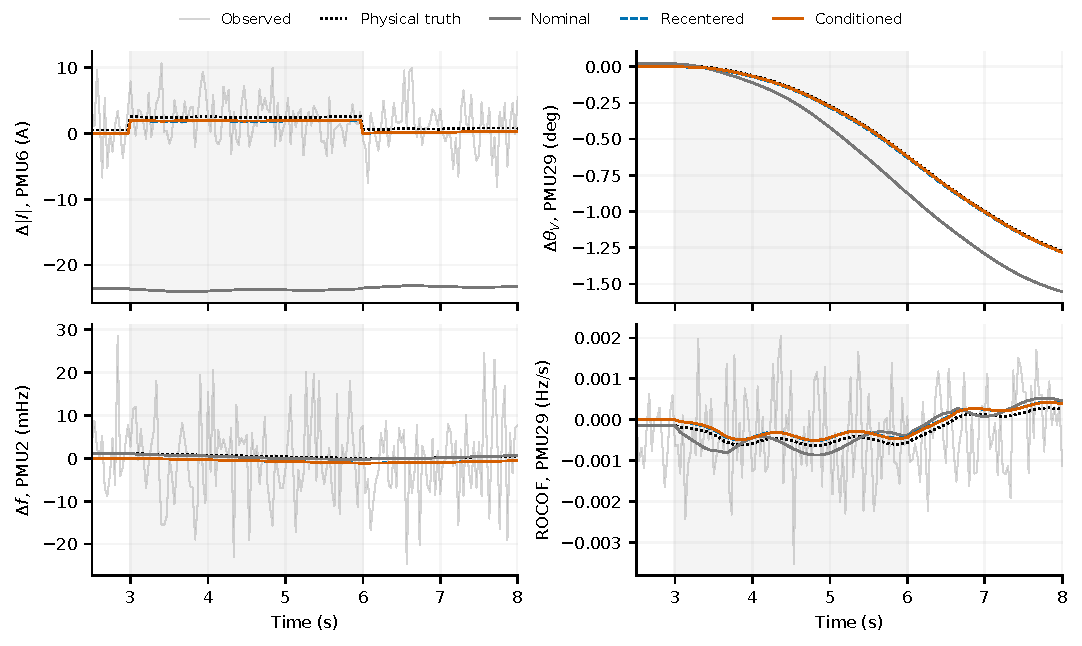
\includegraphics[width=.96\textwidth]{figures/generated/ei_x02_signals.pdf}
\caption{Fixed illustrative test: BUS7, $\eta=+3\%$, load factor $+1\%$,
seed 390502. Gray traces are the delivered PMU observations. Colored curves
use each method's selected source and estimated severity; a no-event
selection keeps its baseline. The dotted black curve is physical truth,
used only for illustration. The plotted channels and case were fixed
without selecting the largest improvement. Shading marks physical ON/OFF
for evaluation.}
\label{fig:ei-signals}\end{figure*}

Paired intervals resample physical test cases, keeping their noise seeds
and methods together. The same three noise seeds are reused across cases;
these intervals describe case variation conditional on those common noise
realizations, not uncertainty over a noise population or transfer to arbitrary
sources or plants. The step-halving checks and all
case outcomes remain in the frozen artifact package. Better fidelity, if
observed, is not sufficient to establish calibrated source probabilities,
all-family diagnosis or a benefit in the unchanged causal campaign.
}{}
\section{Interpretation and Limits}
\label{sec:discussion}

\subsection{Response Fit, Severity and Source Identity}
\label{sec:narrative-information}

A better physical prediction need not produce a better location. Competing
sources may remain similar after their severities and initial conditions
are fitted. For a response $s_h$ at specified severity and context, the
distance to an admitted competitor is
\begin{equation}
 d_h^2=\min_{j\ne h}\ \min_{\beta_j\in\mathcal A_j}
       \|s_h-s_j(\beta_j)\|_{\Sigma^{-1}}^2.
 \label{eq:narrative-separation}
\end{equation}
The set $\mathcal A_j$ fixes allowed signs, severities and nuisance
coordinates. Small distance makes source discrimination noise-sensitive;
it is not a universal error formula or a calibrated decision certificate
\cite{eriksson2013diagnosability,scharf1994matched}.

Three outcomes remain separate: prediction error at a specified physical
source, ranking of competing sources, and uncertainty calibration. A
response improvement establishes the first. It establishes the second only
if source decisions improve under the same observations, horizon and
decision rule. Neither establishes the third automatically. A nonlinear
response comparison is needed before treating a surrogate's residual
confusion as an unavoidable physical limit.

The supplementary archive retains the earlier state-reconstruction and
simultaneous-load studies, with their separate observation contracts and
prior-normalization qualification. Their known-onset scores are not
combined with the causal results here. In particular, recovering hidden
voltages does not certify the source that moved them.

To first order, a component of the context derivative parallel to a nominal
source signature can be absorbed by fitting a different severity. Correct
source ranking can therefore coexist with biased intensity. Components
orthogonal to that signature cannot be removed by this rescaling. This
explains why source accuracy can reach a test ceiling while response and
severity errors still distinguish the models; it is a standard projection
argument, not a new identifiability theorem.


\subsection{Operational Meaning and Scope}
The physical distinction underlying the stream method is simple:
restoration changes an input or topology, but does not erase the machine
state. Retaining that state lets recovery compete with a new intervention.
The development comparison also shows why alarm count and timely location
must be reported together. Stricter admission can suppress extras while
rejecting a real load. The existing admission ablation does not isolate
the contribution of every recovery-memory operation.

\IfFileExists{generated/ei_x02_macros.tex}{The signature experiment addresses
a different source of error. Its corrected variants receive the same
pre-event measurements and offset. Any difference between them therefore
comes from the event--context term and its estimated context, rather than
a privileged baseline or longer window. This isolates the tested response
approximation, but not an improvement of the unchanged causal detector.
Known timing, one scalar context and four load sources make it a controlled
component test.}{Changing an operating reference can also leave the event
response misspecified. A matched signature experiment is needed to
distinguish that error from an onset or recovery failure.}

Our construction builds on trajectory-based diagnosis, sequential
likelihoods and multiple-model filtering. Their general principles are not
new contributions here. The methodological claim concerns the specified
competition among intervention and recovery histories; the experiments
measure its operational behavior. Numerical superiority is claimed only
where a common-data comparison supports it, not over Warner or other
procedures that were not executed.

The continuous catalog contains nine load buses and nine lines and requires
an intervention-free startup. Missing PMUs, unknown families, source-excluded
causal transfer and field operation are untested. F01 retains a provisional
BUS5 current terminal and excludes BUS39 current angle. Agreement with
this research model does not establish the producer's CT placement or
exact reproduction of RAW0001. Local predictors, history pruning, covariance
approximations and fitted startup parameters also limit probability claims.

F01's noise port applies temporal and cross-PMU structure within each
signal family. Its archived cross-family factor covariance is not applied,
and frequency/ROCOF noise is added after phase estimation. The inference
comparison therefore concerns this declared simulator, not the complete
dependence structure of a physical PMU installation.

The two ExtraTrees adapters are particular frozen implementations. Their
load-transfer failure does not rule out learned load diagnosis or establish
a better official hackathon score. Chen's eligible test concerns persistent
line openings; its F01 adapter has DC/white-injection assumptions that do
not capture all instrumental effects. Its mismatches and censored decisions
remain part of the comparison.

A further extension would integrate a vector of pre-event context uncertainties rather
than substituting a point estimate. A local Gaussian approximation gives
\begin{equation}
 V_h(a)=\Sigma_W+J_{\eta,h}(a)P_{\eta,\tau}J_{\eta,h}(a)^\top.
 \label{eq:context-conditioned-extension}
\end{equation}
Its determinant belongs in the likelihood. The covariance must be
calibrated without absorbing the response directions that distinguish
sources. Neither the stream scores nor the signature test validate this
joint extension, an unrestricted multi-source estimator or an optimal
filter. Those questions require their own fixed comparisons.

Finally, processing reports causally is not proof of real-time throughput.
Observation time, computation and queue delay must be measured separately.
The present implementations remain research inference services rather
than validated protection or control systems.

\section{Conclusion}
\label{sec:conclusion}

We formulated sparse-PMU event attribution through competing physical
histories. Load/line predictors start from estimated past states and retain
the cause of the response after restoration. Active mass $M$ and its
increment $\Delta M$ expose the changing explanation rather than replacing
the physical dynamics.

\IfFileExists{generated/c01_macros.tex}{The independent continuous
evaluation gives \COneMixTimely{}/\COneMixTotal{} timely family/source
decisions with \COneMixExtras{} extra alarms for the mixture, and
\COneNomTimely{}/\COneNomTotal{} with \COneNomExtras{} for nominal.
Stratified results and paired intervals determine where each choice is
useful.}{In completed development streams, the mixture obtains
\ContMixTimely{}/\ContMixTotal{} timely family/source decisions with
\ContMixExtras{} extra alarms. Nominal gains one timely decision at a
higher alarm burden. Independent confirmation remains in progress.}

\IfFileExists{generated/ei_x02_macros.tex}{The controlled load test distinguishes reference correction from signature conditioning. The mixed term reduces response error and median relative severity error, but does not establish a directional improvement in joint source decisions. This component result does not change the frozen causal method.
}{}

The result is a specified physical attribution procedure and a testable
separation of recovery, reference error and source discrimination. Its
scope remains the declared simulation contracts. It does not establish
all-family diagnosis, universal source recovery, calibrated probabilities
or real-time deployment.


\section*{Acknowledgment}
OpenAI Codex assisted with drafting and restructuring the main text,
LaTeX preparation, and plotting and execution-infrastructure code.
The authors retain responsibility for the scientific content, verification,
and final submission.
\FloatBarrier
\bibliographystyle{IEEEtran}
\bibliography{references}

\EOD
\end{document}
